\section{Transvertern}
\index{transverter}
\index{mottagare!transverter}

\begin{figure}
  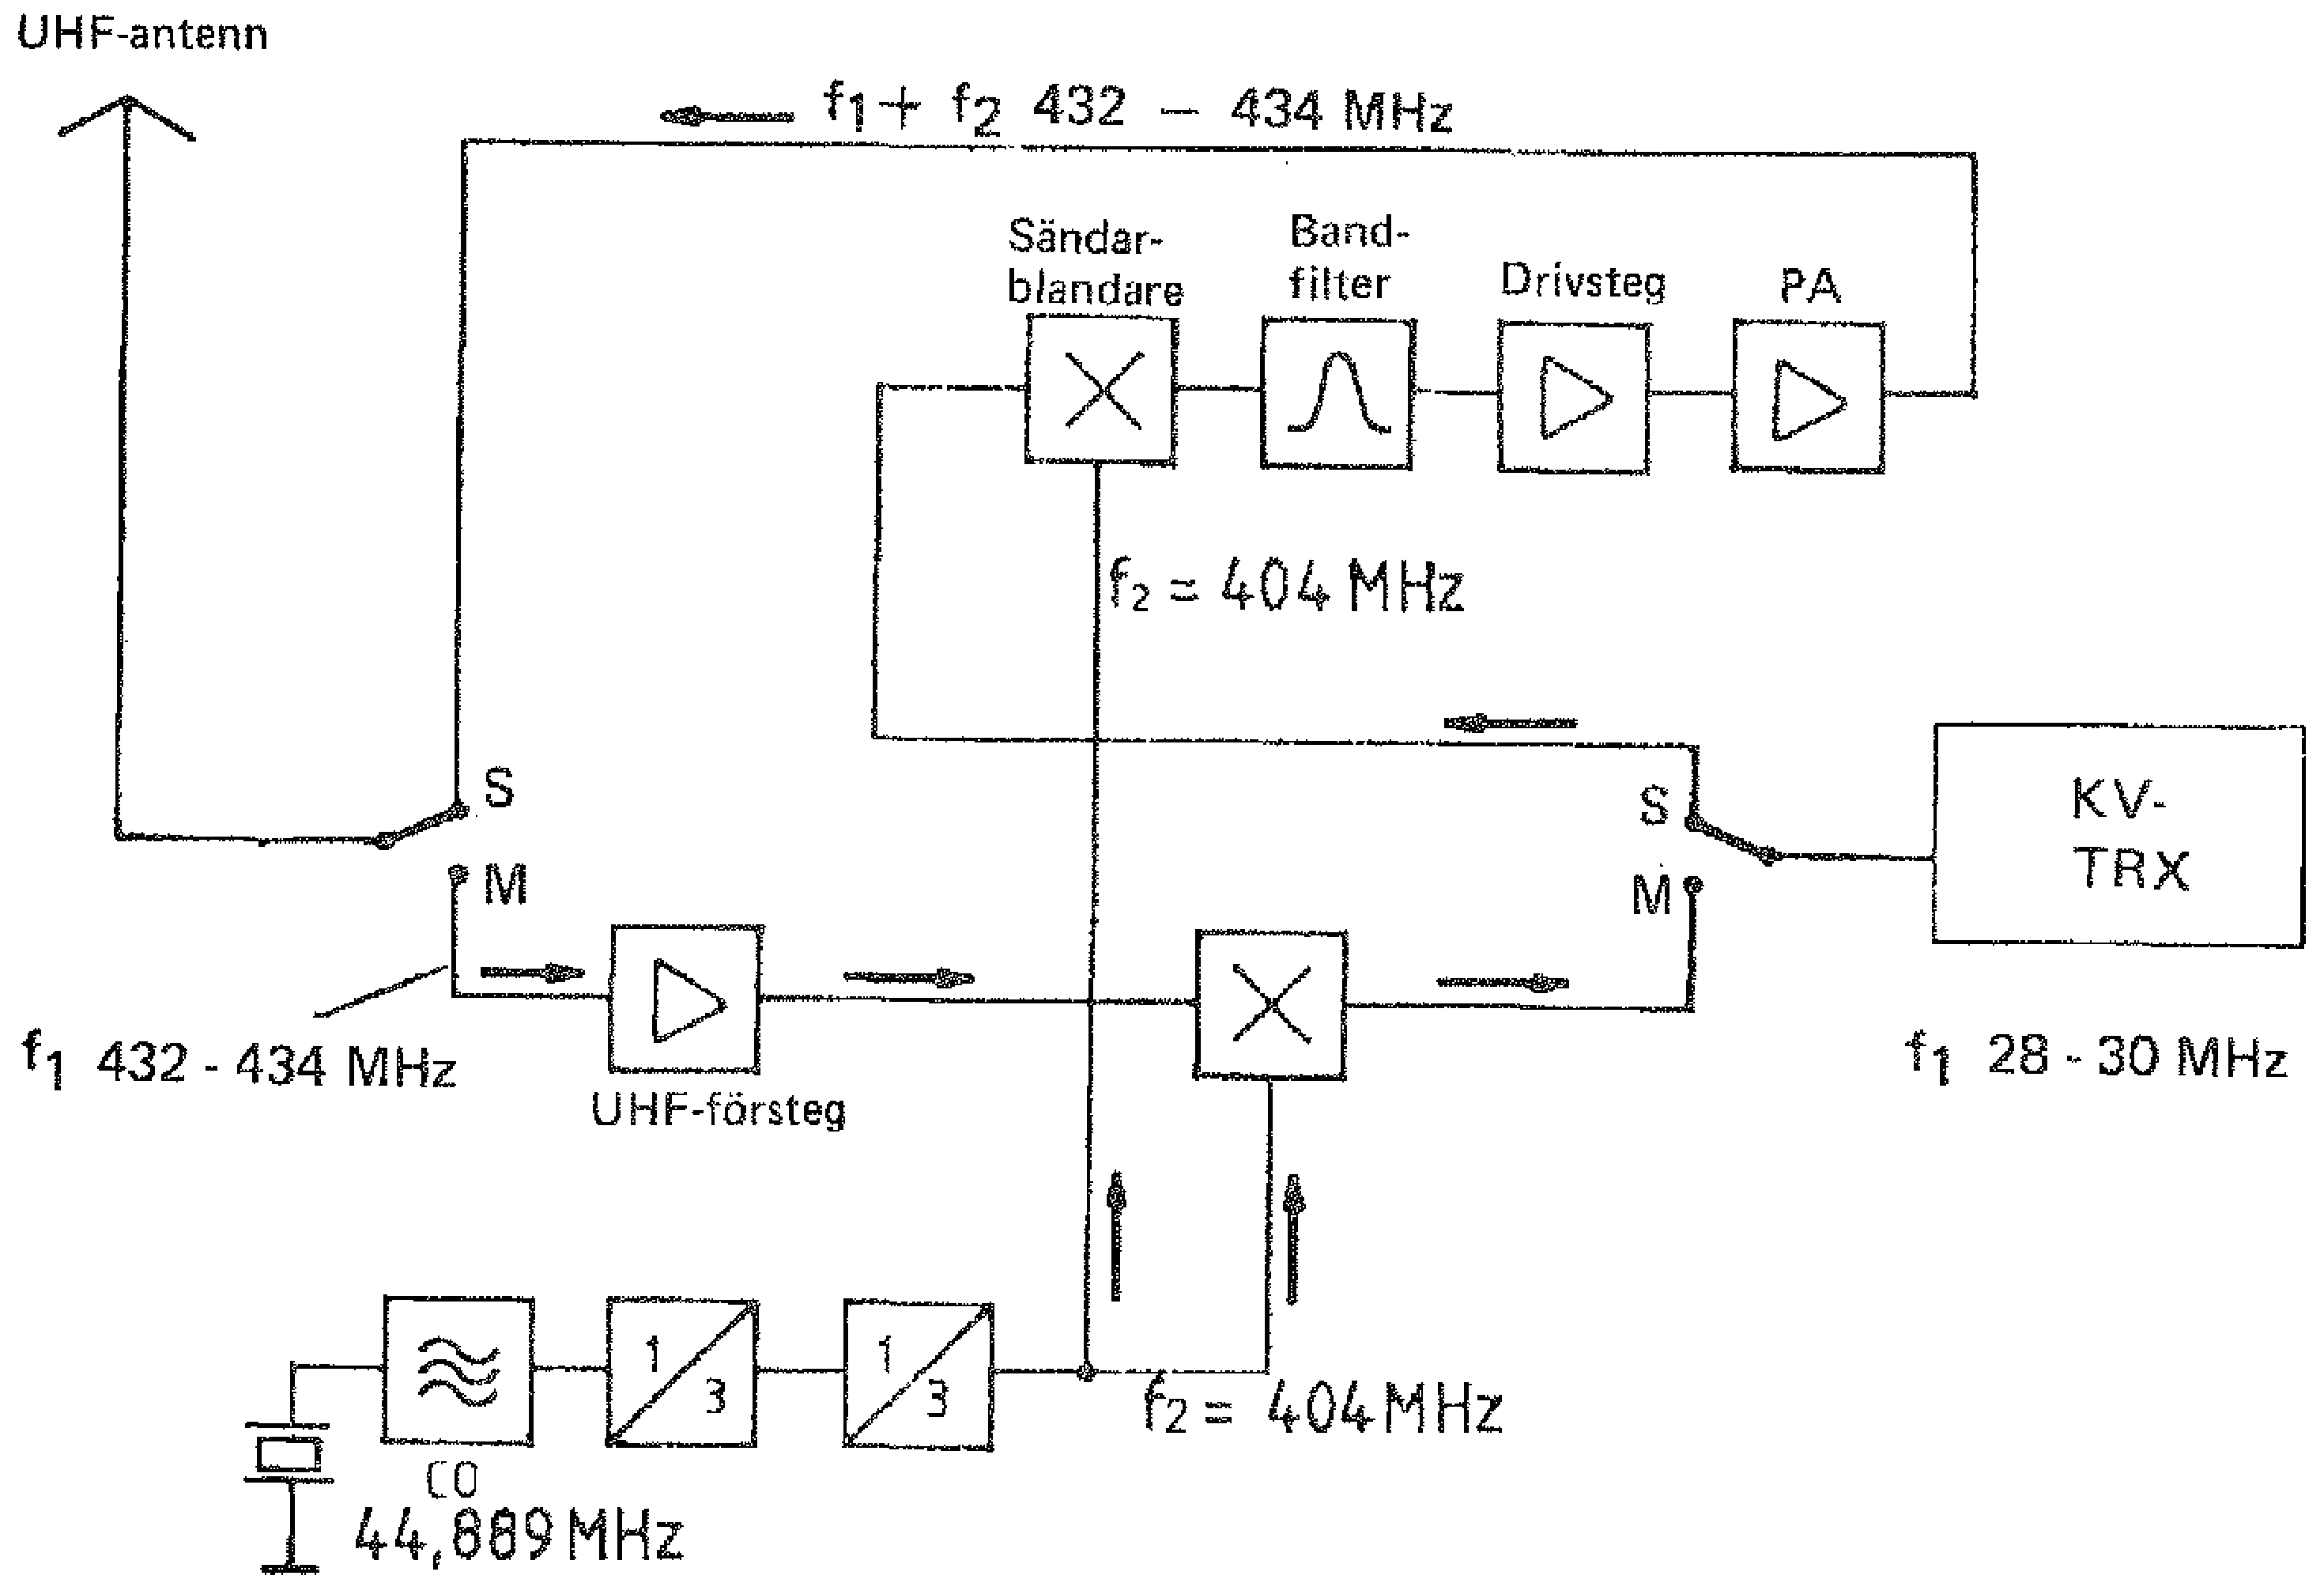
\includegraphics[width=\textwidth]{images/cropped_pdfs/bild_2_4-19.pdf}
  \caption{Transverter mellan UHF och KV}
  \label{fig:bildII4-19}
\end{figure}

En transverter (\emph{trans}sceiver-con\emph{verter}), är en kombinerad
frekvensomvandlare för både sändning och mottagning, som illustreras i
bild \ref{fig:bildII4-19}.
Den förflyttar både mottagnings- och sändningssignaler mellan två
frekvensområden.

Transvertern är ett bra exempel på hur samma teknik kan användas både
i mottagare och sändare.
Om till exempel en KV-transceiver redan finns, kan både mottagning och sändning
ordnas även på andra band med en transverter som tillsats.

\textbf{Exempel:}
En konverter förflyttar de mottagna UHF-signalerna till kortvågsområdet.
Som huvudmottagare används en KV-transceiver i mottagningsläge.
Konvertern kan utökas till att även fungera vid sändning och kallas då
transverter.
Med KV-transceivern i sändningsläge flyttas dess signaler till UHF-området
genom blandning i transvertern av KV-signalen och en multiplicerad signal
från en lokaloscillator (LO).
Den önskade blandningsprodukten i UHF-området filtreras fram och förstärks i
efterföljande driv- och slutsteg.
Samma frekvensmultipliceringskedja efter kristalloscillatorn CO kan användas
för sändning och mottagning.

Fördelen med en transverter är att kostnaden för en sådan är låg jämfört med
den för en komplett transceiver även för det tillkommande bandet.
Förutsättningen är att en transceiver för något band redan finns.
Nackdelen är att den befintliga transceivern inte samtidigt kan användas på
några andra frekvenser än de som används för tillfället.
